\chapter[Message Passing]{Message Passing \\ \Large \textnormal{Group Milestone}}

\section{Introduction}

\label{chapter:mp}
Message passing and inter-process communication (IPC) are vital within Barrelfish, as they enable efficient and secure communication between different system components. Message passing promotes modularity, encapsulation, and clear separation of concerns. It allows independent development, reduces dependencies, and facilitates communication across platforms. In Barrelfish, message passing is integral to achieving isolation, fault tolerance, and scalability. This chapter explores the mechanisms, communication models, and design principles behind message passing in Barrelfish, focusing on the different abstraction levels and the differences between intra- and inter-core communication.

\section{Light-weight Message Passing}
The most fundamental way for passing messages between processes is by using the light-weight message passing (LMP) facilities provided by the kernel. With each message, up to 64 bytes and one capability can be transferred using LMP.

For LMP, the process of sending and receiving data is entirely handled by the kernel, and hence not very interesting. The connection setup, however, is not entirely trivial.

When a process is spawned, we initialize an LMP endpoint in the spawning init process, and pass a capability to this endpoint at a well known location in the spawned process' CSpace. At that point, the spawned process can initialize its own endpoint and can already send messages to init. However, because the process only sets up its endpoint after being spawned, init does not automatically have access to it, and can hence also not send any replies to the process.

We solve this by adding a lazy setup procedure to our LMP channel: Just before the first rpc request is made by the client, a message containing only the endpoint capability is sent to the init endpoint. There, a specially registered bootstrap listener finishes the rpc initialization procedure, before finally starting to listen for regular rpc requests.

\section{User-Level Message Passing}
While LMP provides a nice abstraction for sending small messages between endpoints, it is limited in several important ways. One consideration is that the transmission of every single message requires a system call. While this overhead is small, it is becomes significant when processes need to frequently transmit many small messages, for example during I/O workloads.
A much more fundamental limitation, however, is that, because LMP relies on kernel support, and the Barrelfish kernel is local to each processing core of the system, LMP cannot be used to transmit messages between cores.

For these reasons, User-level message passing (UMP) exists as an alternative mechanism for transferring messages between processes. As the name implies, UMP works entirely in user space, through a frame shared between the communicating processes. By reading from and writing to the frame in a coordinated manner, the two processes can send messages bi-directionally.

Figure \ref{fig:rpc:umpchan} illustrates the general setup of the frame used by the UMP channel. The frame is split into two sections, one of which is used by B to send messages to A, and the other for sending messages from A to B. These two sections each form a ring buffer: The sender writes messages to the end of the queue as long as there is enough space, and the receiver reads messages as long as the entries are valid.
\begin{figure}[htp]
    \centering
    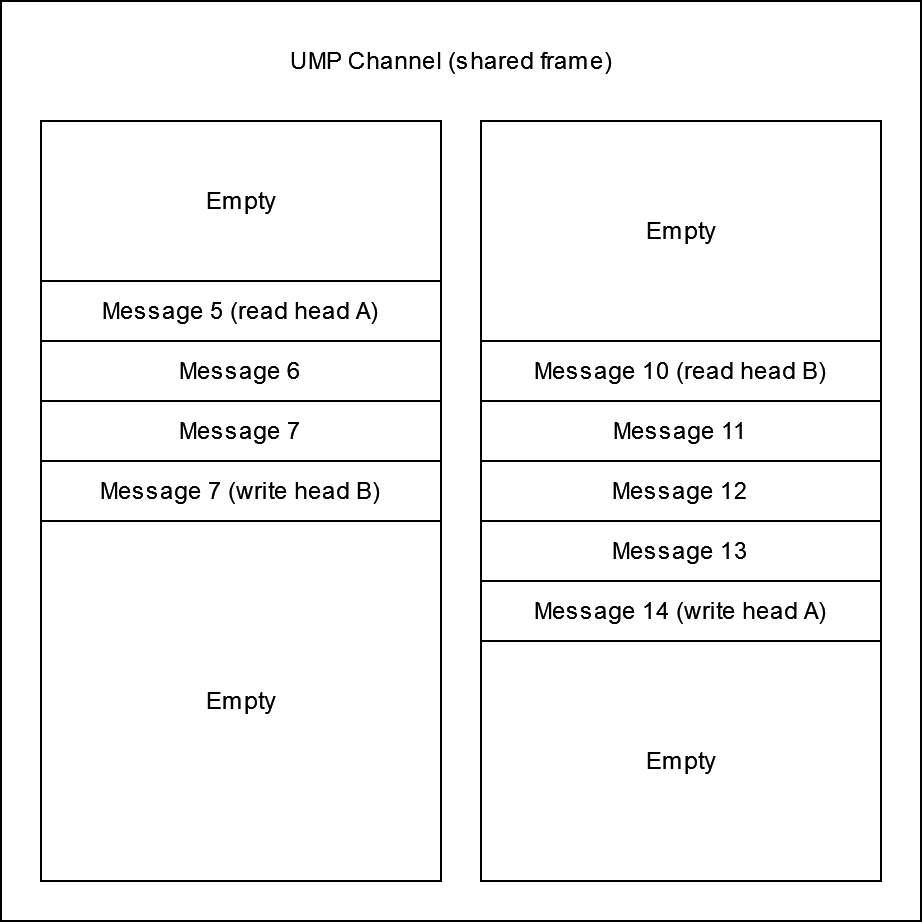
\includegraphics[width=12cm]{images/rpc/ump_chan.png}
    \caption{General structure of a UMP communication channel}
    \label{fig:rpc:umpchan}
\end{figure}

The contents of a single ump message are illustrated in figure \ref{fig:rpc:umpline}. Each message is as large as a single cache line. The first 56 bytes of the message hold the data to be sent, while the last 8 bytes are a control word holding the size of the message data in bytes\footnote{in retrospect, the control word only needs to be a single byte, not eight, as many of the size bits are wasted}, as well as a bit indicating whether the message of the higher-level protocol (discussed in the next section) was fragmented and more data follows in the next message.

\begin{figure}[htp]
    \centering
    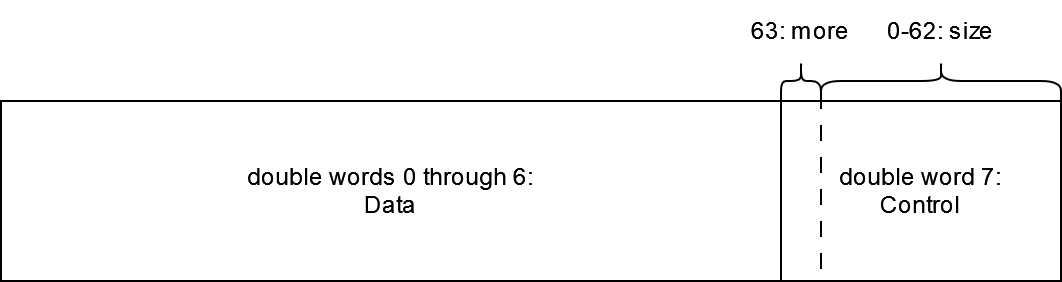
\includegraphics[width=12cm]{images/rpc/ump_line.png}
    \caption{The contents of a single cache line holding a UMP message}
    \label{fig:rpc:umpline}
\end{figure}

Listing \ref{listing:umpsend} shows the process of sending a UMP message on a channel. The ump channel object keeps track of the offset at which the next message should be sent. From there, the process consists simply of copying the data to be sent into the specified slot, followed by updating the control word. Importantly, a barrier is necessary between writing the data and setting the control word, to ensure that the receiver observes the update to the data before it starts reading it. There is no need for a barrier between checking if there is space in the channel and writing to it, as writes are never speculated\footnote{TODO reference to ARM manual}.

\begin{lstlisting}[caption={Sending a UMP message},label={listing:umpsend}]
static inline errval_t ump_chan_send(struct ump_chan* chan, const struct ump_msg* msg) {
    if (!ump_chan_can_send(chan)) {
        return LIB_ERR_UMP_CHAN_FULL;
    }
    
    // writes are never speculated, hence no barrier is necessary
    
    struct ump_line* line = chan->send.buf + chan->send.offset;
    memcpy(line->words, msg->data, msg->size);

    uintptr_t control = msg->size | (msg->more ? UMP_MSG_MORE : 0);

    // written data must be visible before control word
    dmb();

    line->words[UMP_CONTROL_WORD_IDX] = control;

    chan->send.offset = (chan->send.offset + 1) % chan->send.size;

    return SYS_ERR_OK;
}
\end{lstlisting}

The process of receiving a message is analogous, and shown in listing \ref{listing:umprecv}. We first check if the channel can receive a message, and, if it can, read out the data. We then set the control word to 0 to indicate to the writer that the slot is now clear.

In this case, two barriers are required: The first (on line 12) ensures that the data is not speculatively prefetched before the line is set to be valid by the sender, while the second (on line 17) ensures that the data is fully read before the sender can start writing to it again.
The control data can be read before the barrier because it is a direct data dependency of the condition.

\begin{lstlisting}[caption={Receiving a UMP message},label={listing:umprecv}]
static inline errval_t ump_chan_recv(struct ump_chan* chan, struct ump_msg* msg) {
    if (!ump_chan_can_recv(chan)) {
        return LIB_ERR_UMP_CHAN_EMPTY;
    }

    struct ump_line* line = chan->recv.buf + chan->recv.offset;
    uintptr_t control = line->words[UMP_CONTROL_WORD_IDX];
    msg->size = control & UMP_MSG_SIZE_MASK;
    msg->more = control & UMP_MSG_MORE;

    // avoid data being prefetched speculatively
    dmb();

    memcpy(msg->data, line->words, msg->size);

    // data must be read before clearing control word visible to writer
    dmb();

    // clear control word after reading data
    line->words[UMP_CONTROL_WORD_IDX] = 0;

    chan->recv.offset = (chan->recv.offset + 1) % chan->recv.size;

    return SYS_ERR_OK;
}
\end{lstlisting}

Finally, listing \ref{listing:umpcheck} shows how a message is defined to be (in)valid: If the control word is zero, the slot is empty and can be overwritten. On the other hand, if the control word is nonzero, it contains a message which can be read out. Note that this means that messages of length 0 are not supported, as that would imply the control word to be  zero for a valid message.
\begin{lstlisting}[caption={Checking if an entry is (in)valid},label={listing:umpcheck}]
static inline bool ump_chan_can_send(struct ump_chan* chan) {
    struct ump_line* line = chan->send.buf + chan->send.offset;
    return line->words[UMP_CONTROL_WORD_IDX] == 0;
}

static inline bool ump_chan_can_recv(struct ump_chan* chan) {
    struct ump_line* line = chan->recv.buf + chan->recv.offset;
    return line->words[UMP_CONTROL_WORD_IDX] != 0;
}
\end{lstlisting}

\section{Transport Layer}
To mitigate the additional complexity that arises when having to manage several different protocols at a time, as well as to avoid having to manage message fragmentation and metadata when implementing remote procedure calls and their respective handlers, LMP and UMP are abstracted under a common interface with message semantics. This interface is designed to allow for both blocking and non-blocking communication, to fragment and reassemble both the data and the capabilities being sent, as well as to almost completely abstract away the difference between LMP and UMP.

Once an rpc structure has been initialized using one of the LMP- or UMP-specific methods, there are several functions which can be used to interact with it to engage in communication.
The most important of these are 
\begin{enumerate}
    \item \texttt{aos\_rpc\_send\_with\_handler} and
    \item \texttt{aos\_rpc\_recv\_with\_handler}
\end{enumerate}
Both of these functions take as arguments a pointer to the rpc structure on which they are being invoked, as well as a a closure which is to be called once the respective operation finishes. \texttt{struct aos\_rpc} has members which describe the data to be sent, or the buffer to use when receiving data. These must be set before calling any functions for sending or receiving data.

Even though they are the most important interface for sending and receiving data through rpc, the above functions don't actually do much work themselves. Instead, they simply remember the corresponding handler closure in \texttt{struct aos\_rpc}, and then register an event handler for the underlying channel. Listing \ref{listing:sendhandler} shows the handler for sending messages. When the send handler is called, it tries to send a fragment of the message by using \texttt{transport\_try\_send}. This also updates internal offset values in \texttt{struct aos\_rpc}. Then, if more parts of the message remain to be sent, the handler is re-registered and, because the internal state was updated, on the next invocation, it will send the next part of the message. If no more parts of the message remain, the sending state is reset, and the handler which was originally set in \texttt{aos\_rpc\_send\_with\_handler} is invoked.

The interface for receiving data is completely analogous.

\begin{lstlisting}[caption={Send handler registered on waitset},label={listing:sendhandler}]
static void transport_send_handler(void *arg)
{
    errval_t        err = SYS_ERR_OK;
    struct aos_rpc *rpc = arg;

    bool more = false;
    err       = transport_try_send(rpc, &more);

    if (err_is_fail(err) 
        && !(lmp_err_is_transient(err) 
        || ump_err_is_transient(err))) {
        USER_PANIC_ERR(err, "transport_try_send");
    }

    if (more) {
        transport_register_send(
            rpc, MKCLOSURE(transport_send_handler, arg));
    } else {
        // reset send state
        rpc->send_offset      = 0;
        rpc->send_caps_offset = 0;
        if (rpc->send_handler.handler) {
            rpc->send_handler.handler(rpc, rpc->send_handler.data);
        }
    }
}
\end{lstlisting}

Listing \ref{listing:sendblocking} shows how \texttt{aos\_rpc\_send\_with\_handler} can be used to implement a blocking send operation, such as the one used for RPC calls, discussed in section \ref{section:rpc:rpc}. It consists of three main components:
\begin{enumerate}
    \item The data and capabilities which will be sent is set up in the rpc structure.
    \item A send operation is issued on the rpc structure, with a handler that updates a flag once the operation finishes.
    \item Events are dispatched on the waitset associated with the rpc structure until the closure signals that the send operation has concluded.
\end{enumerate}

\begin{lstlisting}[caption={Using \texttt{aos\_rpc\_send\_with\_handler} for a blocking send implementation},label={listing:sendblocking}]
static void _blocking_closure(struct aos_rpc *rpc, void *data)
{
    (void)rpc;
    *(bool *)data = false;
}

errval_t aos_rpc_send_blocking_varsize(struct aos_rpc *rpc, const void *buf, size_t size,
                                       struct capref *capbuf, size_t capsize)
{
    errval_t err = SYS_ERR_OK;

    err = _lmp_init_late_client(rpc);
    if (err_is_fail(err)) {
        return err;
    }

    // set the data to be sent
    rpc->send_buf.data = (void *)buf;
    rpc->send_size     = size;
    rpc->send_buf.size = size;

    // set capabilities to be sent
    rpc->send_buf.caps  = capbuf;
    rpc->send_caps_size = capsize;

    bool waiting = true;
    aos_rpc_send_with_handler(
        rpc, MKHANDLER(_blocking_closure, &waiting));
    // block until the send operation has been finished
    while (waiting) {
        err = event_dispatch(rpc->waitset);
        if (err_is_fail(err)) {
            return err;
        }
    }

    return err;
}
\end{lstlisting}

\section{A detour: The init process and blocking operations}
\label{section:rpc:initnoblock}
In our design, each core's respective init process is the coordinator through which almost all operations are performed, from memory allocation to process management or file system operations. They are either performed in-process (by using the RAM allocator within the init process, for example) or forwarded to another process for handling, for example for performing operations on  the file system.

Because most of init's work consists of communication (either with user processes or the other init process), we decided on a fully asynchronous and non-blocking design. There is only a single thread which is dispatching events on the default waitset. When an operation needs to wait until a later point in time, a callback is registered and other operations are executed in the meantime.

This design has several advantages, the most obvious being that we are able to completely avoid any synchronization through mutexes, condition variables, etc. Basically, all perils of multi-threaded programming are avoided. Furthermore, we also avoid the need for keeping around waiting threads to handle events for user processes. It may be reasonable to say that this is the leanest-possible design for a centralized init process. This, however, means that it is of paramount importance to ensure that \textit{no} blocking operations are used in init

There are, however, also issues with our approach: Asynchronous programming is difficult when the programming language provides absolutely no language features to facilitate it. Especially for operations which may need to suspend multiple times, keeping around local variables in special \texttt{struct}s is tedious and error-prone, and manually registering callbacks quickly obscures the actual flow of control.

\section{Remote Procedure Calls}
\label{section:rpc:rpc}
Between user processes and the respective init processes on the same core, we employ an interface structured around blocking remote procedure calls. Importantly, these calls are \textit{only} blocking to the user processes. The init process, as stated previously, never blocks.

When a process is spawned, a communication channel is automatically set up between the spawned process and the init process executing the spawn. In fact, the structure keeping track of the communication state between init and the spawned process is part of the \texttt{struct spawninfo} which keeps track of various kinds of state related to the process. The fact that there is only a single \textit{blocking} communication channel between each process and init naturally implies that all RPCs originating from a single process are serialized, and cannot occur concurrently. We will discuss this in more detail when talking about the limitations of our system in section \ref{section:rpc:limitations}.

Because all RPCs are issued through a single communication channel, a common protocol is required such that the init process knows which handler to call when a request arrives.
We achieve this by using a hierarchy of structs, with an enumerator containing all possible request types at the base level. Listing \ref{listing:rpcstruct} shows an excerpt of this hierarchy. It also highlights how flexible array members can be used for sending arbitrarily large messages (useful for sending strings, for example) across the rpc channel.

\begin{lstlisting}[caption={A hierarchy of request types},label={listing:rpcstruct}]
struct aos_generic_rpc_request {
    enum {
        AOS_RPC_REQUEST_TYPE_MEMSERVER,
        AOS_RPC_REQUEST_TYPE_TERMINAL,
        /* ... */
        AOS_RPC_REQUEST_TYPE_PROC_MGMT,
    } type;
};

struct aos_proc_mgmt_rpc_request {
    struct aos_generic_rpc_request base;
    enum {
        AOS_RPC_PROC_MGMT_REQUEST_SPAWN_CMDLINE,
        AOS_RPC_PROC_MGMT_REQUEST_STATUS,
        /* ... */
        AOS_RPC_PROC_MGMT_REQUEST_NAME,
    } proc_type;
    coreid_t core;
};

struct aos_proc_mgmt_rpc_spawn_request {
    struct aos_proc_mgmt_rpc_request base;
    char cmdline[];
};
\end{lstlisting}

\subsection{Performing the Call}
From the perspective of a user process, an rpc call consists of the following steps:
\begin{enumerate}
    \item Marshal the arguments into the appropriate structure
    \item Send the structure (and capabilities, if any need to be sent) into the channel using the blocking send operation.
    \item Receive the response from init using a similar blocking receive operation.
    \item Unmarshal the return values and return them to the original caller.
\end{enumerate}
During steps 2 and 3, the user thread making the request becomes blocked. While other user threads may still make progress during this time, no rpcs can be issued concurrently.

\subsection{Handling the Call}
Because init must never block, it cannot use blocking receive operations to wait for RPC requests from a user process to arrive. Instead, it uses \texttt{aos\_rpc\_recv\_with\_handler} to defer until a message actually arrives from the process. Even though there may be many processes, each with their own rpc endpoint, because all are registered on the same waitset which is being continuously dispatched on, init is able to handle requests from all user processes concurrently.

At the core of the rpc system lies the handler closure registered using the previously mentioned receive call. It receives as arguments the message that was received, as well as a handle to the rpc endpoint to which the reply should be sent. When handling rpc requests, there are generally two cases of differing complexity.

In the simplest case, the request can be processed and a reply can be sent \textit{immediately}, without any sort of waiting operation required. In this case, a reply can be sent using \texttt{aos\_rpc\_send\_with\_handler} directly from the handler function. This is the case for many simpler rpc requests, for example memserver requests on core 0.

Things get more complicated when the reply cannot be sent immediately, such as when waiting for a process to terminate. Because init is non-blocking, the handler function cannot simply wait until the target process terminates: This would block the system until that point, and would probably cause a deadlock if the waited-for process also tried to make an rpc. Instead, a callback is registered registered within the process management system to be called when the target process terminates. This callback will then send the actual reply to the original caller. Because the stack frame of the handler will already be long gone, it is important to preserve necessary information accross this suspension point.

For handling requests concerning distributed capabilities, up to three suspensions may be required to handle a single call (wait until capability is unlocked, wait until revoke finishes on other core, wait until revoke finishes on own core). Due to the lack of asynchronous programming support in C, this process quickly becomes tedious.

\section{Asynchronous Message Passing}
\label{section:rpc:async}
Some user requests require communication between the init processes on the two cores. Because only a single communication channel is available, and the init processes must be non-blocking, a different communication system was required for cross-core synchronization. The main requirement for this system is that requests can "overtake" each other: A short request which can be executed and responded to immediately should not block when waiting for a long-running request such as a \texttt{wait} operation. This is best explained in an example:

Imagine two processes, \texttt{p0.0} and \texttt{p0.1}, both on core 0. Now, \texttt{p0.0} makes a \texttt{wait} rpc request for a process on another core. The request will first be sent to init on core 0, which will forward it to core 1, where a callback will be registered in the process management system. Now, \texttt{p0.1} performs a \texttt{cap\_delete} operation which needs to synchronize across cores. 
We desire our cross-core rpc system to be flexible enough to allow
\begin{itemize}
    \item the synchronization request to be made before the wait request has returned.
    \item a reply to the synchronization request to be sent before the wait request has been replied to.
    \item core 1 to issue requests concurrently to handling requests coming from core 0.
\end{itemize}
Neither of these requirements are satisfied by the rpc system described previously.

For this purpose, we devised the \texttt{async\_channel}. It has a very simple interface, consisting of the two functions shown in listing \ref{listing:asyncinterface}.

\begin{lstlisting}[caption={The interface for \texttt{async\_channel}},label={listing:asyncinterface}]
void async_init(struct async_channel *async, struct aos_rpc *rpc,
                async_request_handler handler);
void async_request(struct async_channel *async, void *data, 
                   size_t size, struct capref *capv,
                   size_t capc, async_callback callback, 
                   void *meta);
void async_respond(struct async_channel *async, 
                   struct response *res);
\end{lstlisting}

An \texttt{async\_channel} is initialized on top of a standard \texttt{aos\_rpc} instance. In our implementation, this is always the cross-core channel communicating through UMP. Similarly to the standard rpc server interface, a handler function is also passed upon initialization. This function is called with the request parameters whenever a request arrives, and should schedule \texttt{async\_respond} to be called at some point in the future. Once the response arrives, the \texttt{async\_callback} provided in the initial request is called.

\subsection{Design Details}
Because there is only one cross-core channel, but requests and responses may originate from either core, we multiplex requests and responses on a single communication channel. Furthermore, we allow responses to later requests to be sent before responses to earlier requests. 

This is visually illustrated in figure \ref{fig:rpc:asyncchan}: Core 0 is sending requests with id 13 and 14, while a response to a request issued by the other core is interspersed in the middle. On the other hand, core 1 is replying to requests 2 and 9 out of order, on the same channel used for sending request 12.

\begin{figure}[htp]
    \centering
    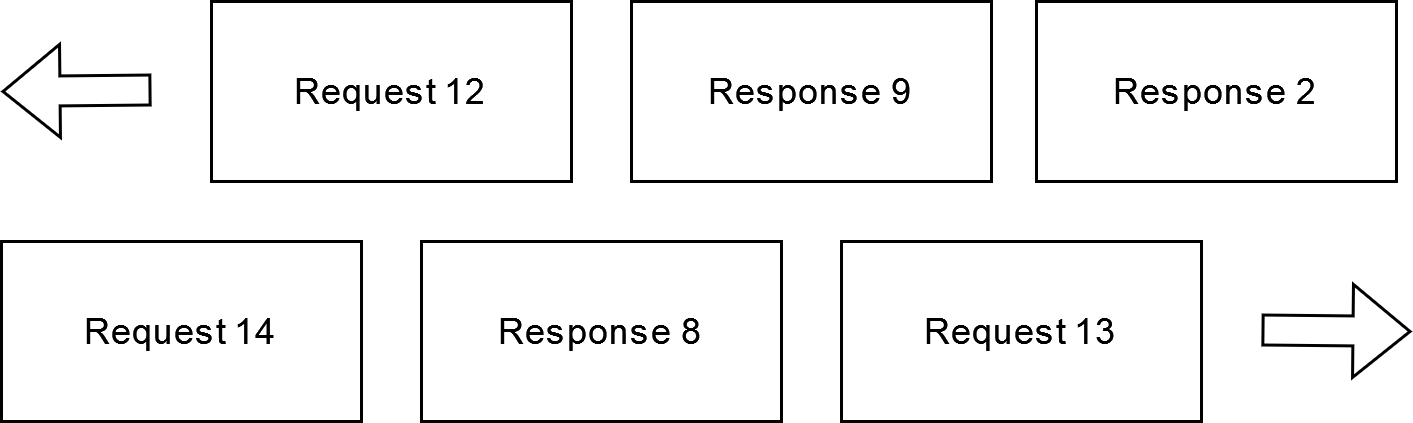
\includegraphics[width=12cm]{images/rpc/async_channel.png}
    \caption{Multiplexed and out-of-order requests and responses}
    \label{fig:rpc:asyncchan}
\end{figure}

\subsection{An Example Request}
\label{subsec:rpc:examplereq}
Let us now consider the life cycle of an example request.
\begin{enumerate}
    \item The request is issued using \texttt{async\_request}. The function allocates a request queue node and appends it to the queue of pending requests of the channel. 
    \item Once it is at the head of the queue, the request is dequeued and sent across the underlying communication channel. Importantly, the request node is \textit{not deallocated}.
    \item The request arrives on the other core, a response object is allocated, and the handler function is called with the data and the response object.
    \item At some point in the future, \texttt{async\_respond} is called on the response object. It is appended to the response queue of the channel.
    \item Once the response is at the head of the queue, it is sent across the channel and the object is deallocated.
    \item The response arrives on the other core, and the handler function provided during the initial request is called.
    \item The original request object is deallocated.
\end{enumerate}

Most steps of this process are straightforward: Sending and receiving messages simply uses \texttt{aos\_rpc\_send\_with\_handler} and \texttt{aos\_rpc\_recv\_with\_handler}, where the respective handler functions simply dequeue more messages or call the handler function registered on the channel. However, there is one significant design question remaining: When a response arrives, how do we find the callback provided during the initial request?

A possible solution would be to use a hash map and associate each request with an identifier. Then, the response simply needs to carry the same identifier as the request, and the data for the correct request can be retrieved. However, because both ends of the communication channel are trusted, we can actually use a much simpler and efficient solution, as shown in listing \ref{listing:asyncmessage}: We simply pass along the address of the request structure allocated in the first step of the \texttt{async\_request}, as explained in \ref{subsec:rpc:examplereq}. This same address is also returned in the response. Then, once a response arrives, we can directly call the handler. The entire process is shown in listing \ref{listing:asyncrecvhandler}.

\begin{lstlisting}[caption={The message type used on the async channel},label={listing:asyncmessage}]
struct async_message {
    struct request     *identifier;
    enum async_msg_type type; // ASYNC_RESPONSE or ASYNC_REQUEST
    size_t              size;
    size_t              capc;
    char                data[];
};
\end{lstlisting}

\begin{lstlisting}[caption={Propagating and directly accessing message identifiers},label={listing:asyncrecvhandler}]
if (msg->type == ASYNC_RESPONSE) {
    // get original request object corresponding to response
    struct request *req = msg->identifier;
    // call callback
    req->callback(req, data, msg->size, capv, msg->capc);
    // free request object
    free(req);
} else if (msg->type == ASYNC_REQUEST) {
    // allocate response
    struct response *res = malloc(sizeof(struct response));
    res->identifier      = msg->identifier;
    res->finalizer       = free_finalizer;
    res->next            = NULL;
    // call handler and give it ref to response
    async->response_handler(
        async, data, msg->size, capv, msg->capc, res);
} else {
    USER_PANIC("Invalid async message type");
}
\end{lstlisting}

\subsection{Sending Capabilities}
Because \texttt{async\_channel} is the only communication channel between the init processes on the two cores, we also use it to implement cross-core capability transfers, as enabled by the distributed capability system (discussed in chapter \ref{chapter:distcap}). This allows requests to be transparently relayed to the other core.
This functionality is enabled by using \texttt{cap\_transfer\_move} when a message is queued for sending and \texttt{cap\_from\_transfer} when it is received on the other core. A more detailed discussion can be found in chapter \ref{chapter:distcap}.

\section{Retrospective}
\label{section:rpc:limitations}
In our design, the most impactful decision was probably to make init single-threaded, asynchronous and fully non-blocking. In a programming language with strong support for asynchronous operations, such as Rust or Zig, this design would probably be the clear winner: It completely avoids all issues related to thread-level parallelism, eliminates the need for synchronization, and is highly memory-efficient when compared to threads. However, in retrospect, it is not clear whether such a design is the best decision, especially when factoring in the significant cognitive overheads of programming asynchronously in C. We may have been able to achieve a similarly performant implementation by spawning an rpc handler thread in the init process for every user process. 
This, however, would not address the most significant limitation of our system: Only a single rpc can be performed concurrently from each user process. A solution to this would be to leverage the same async channel implementation that we used for cross-core communication for handling communication between user processes and init. While this would introduce additional overheads from dynamic allocations, it would make the system more flexible and capable.
